\documentclass[]{article}
\usepackage{amssymb}
\usepackage{amsmath}
\usepackage{pst-all}
\usepackage[pdftex]{graphicx}
\newcommand{\R}{\mathbb{R}}
\begin{document}
\title{Formulaire physique générale I}
\author{Florian Wauters}
\date{02/12/2020}
\maketitle

\part{introduction}

\begin{tabular}{|c|c|c|c|}
\hline
variables & interaction  & intensité relative & portée \\
\hline
& Forte & 1 & $10^{-15}m$\\
Interaction& Electromagnétique & $10^{-2}$ & $\infty$\\
fondamentale& Faible & $10^{-6}$ & $10^{-17}m$\\
& gravitationelle & $10^{-38}$ & $\infty$\\
\hline

vecteurs & propriétés & formules & autres\\
\hline
&&&\\
$\overrightarrow{A} et \overrightarrow{B}$ & scalaire d'un vecteur & $(\overrightarrow{A} \rightarrow \alpha \overrightarrow{a}, \alpha \in \R)$&\\

&&&\\
& commutative & $\overrightarrow{A} + \overrightarrow{B} = \overrightarrow{B} + \overrightarrow{A}$&\\
&&&\\
& associative & $(\overrightarrow{A}+\overrightarrow{B})+\overrightarrow{C} = \overrightarrow{A}+(\overrightarrow{B}+\overrightarrow{C})$ &\\
&&&\\
& composantes & $\overrightarrow{R_{x}} = \overrightarrow{A_{x}}+\overrightarrow{B_{x}}$&\\

& & $\overrightarrow{R_{y}} = \overrightarrow{A_{y}}+\overrightarrow{B_{y}}$ &\\

&&&\\
& vecteurs unitaires & $||\overrightarrow{i}|| = ||\overrightarrow{j}||=||\overrightarrow{k}||=1$&\\
&&&\\
& vecteur $\overrightarrow{A}$ peut s'écrire & $\overrightarrow{A}=A_{x}\overrightarrow{i} + A_{y}\overrightarrow{j} + A_{z}\overrightarrow{k}$&\\
&&&\\
&norme du vecteur&$||\overrightarrow{A}|| = A = \sqrt{A^{2}_{x}+A^{2}_{y}+A^{2}_{z}}$&\\
&égalité de vecteur & $\overrightarrow{A}=\overrightarrow{B}\Leftrightarrow A_x=B_x \wedge A_y=B_y \wedge A_z=B_z$&\\
&&&\\
&produit scalaire& $\overrightarrow{A}\cdot \overrightarrow{B} = A\cdot B\cdot \cos{\theta}$&\\
&&&\\
&produit vectoriel&$\overrightarrow{A}\times \overrightarrow{B}=A \cdot B \cdot \sin{\theta} \cdot \overrightarrow{u_n}$&\\
&& il est anti-commutatif&\\
&&$\overrightarrow{A}\times \overrightarrow{B}=-\overrightarrow{B}\times \overrightarrow{A}$&\\
&& il est distributif &\\
&&peser a la règle de la main droite&\\
\hline
\end{tabular}
\newpage
\part{cinématique a une dimension}
\begin{itemize}
 \item particule : voiture
 \item système de référence : route
\end{itemize}
Position :

spécifiée en fonction d'une seule coordonnée x\\\\
Mouvement : 

en fontion du temps $x(t)$\\\\
Déplacement :

vecteur a une composante $\Delta \overrightarrow{x} = \overrightarrow{x_f} - \overrightarrow{x_i}$

position initiale $\rightarrow$ position finale

$\Delta x = x_f - x_i$

cette composante peut être nulle, positive ou négative
\\\\
Vitesse Moyenne :

durant un intervalle donné $\Delta t = t_f - t_i$

La formule est $v_{x_{moy}}= \frac{\Delta x}{\Delta t} = \frac{x_f-x_i}{t_f-t_i}$

représentation graphique:\\
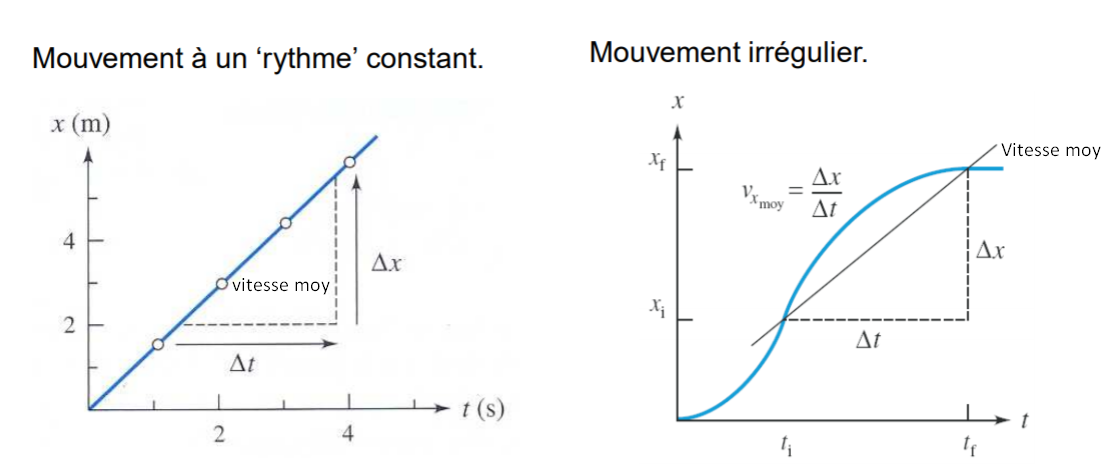
\includegraphics[scale=0.65]{vitesse_moy_graphe.png}\\
\newpage
Vitesse instantanée :

$v(t)=\displaystyle \lim_{\Delta t \to 0}\frac{\Delta x}{\Delta t}$

$v(t)\equiv x = \frac{dx}{dt}$

représentation graphique:\\
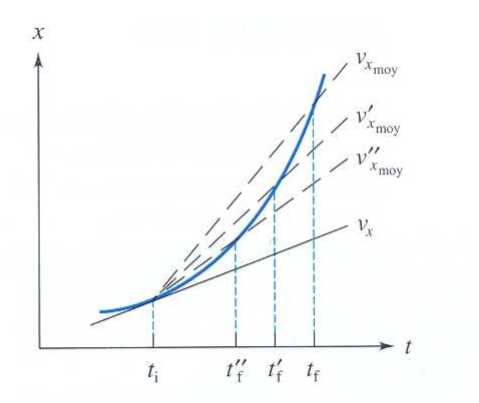
\includegraphics[scale=0.65]{vitesse_inst_graphe}\\
Accélération moyenne :

taux de variation de vitesse $\Delta V$ sur un temps $\Delta t$

$a_{x_{moy}} = \frac{\Delta v_x}{\Delta t}$\\\\
Acceleration instantanée :

dérivée de la vitesse par rapport au temps t :

$a(t) = \displaystyle \lim_{\Delta t \to 0}\frac{\Delta v}{\Delta  t}$\\\\
\newpage
Utilisation des aires :\\
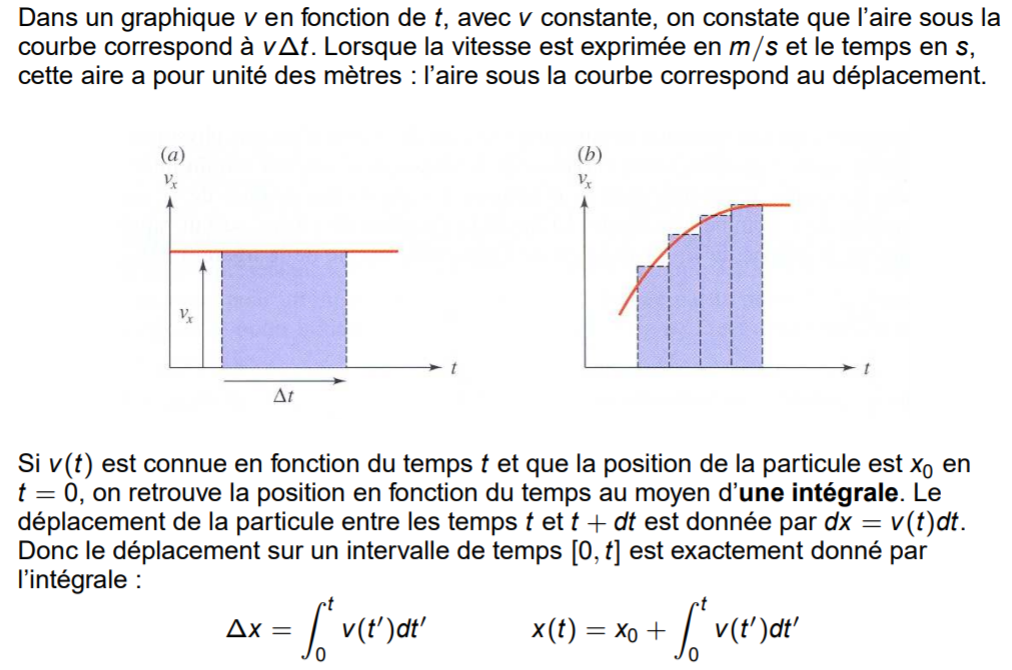
\includegraphics[scale=0.65]{utilisation_aires}\\
On peut donc écrire la variation de position et de vitesse comme\\

$dx = v_xdt$\\

$dv = a_xdt$\\

donc :

\indent \indent $\Delta x = x(t) - x(0) = \displaystyle \int^t_0 v_x(t')dt'$\\

\indent \indent $\Delta v_x = v_x(t) - v_x(0) = \displaystyle \int^t_0 a_x(t')dt'$\\

A vitesse constante, l'acceleration est nulle :\\

\indent \indent $a = \frac{dv}{dt}=0$

On peut alors retrouver l'équation du déplacement de la particule :\\

\indent \indent $x(t)= x_0 + \displaystyle \int^t_0 v(t')dt' = x_0 + v\int^t_0 dt' = x_0 + vt$\\

c'est l'équation du déplacement en MRU

\newpage

Equation à accélération constante :\\

\indent \indent $\Delta v = \displaystyle \int^t_0 a(t')dt'$

donc\\

\indent \indent $v(t) = v_{x0} + \displaystyle \int^t_0 a(t')dt' = v_{x0} +a \int^t_0 dt' = v_{x0} + at$

la position de la particule est donnée par :\\

\indent \indent $x(t) = x_{0} + \displaystyle \int^t_0 v(t')dt' = x_0 + \int^t_0 (v_{x0}+at')dt' = x_0 + v_{x0}t + \frac{at^2}{2}$\\

Par conséquent on peut résumer :\\

\indent \indent $x(t) = x_0 + v_{x0}t + \frac{at^2}{2}$\\\\
\indent \indent $v(t) = v_{x0} + at$\\

Ce sont les équation de la vitesse et de la particules en MRUA et montrent que :

\begin{itemize}
  \item la variation de vitesse de la particule est linéaire 
  \item la variation de déplaceent de la particule est quadratique
\end{itemize}

En combinant ces deux équation on trouve une nouvelle équation :\\

\indent \indent $v^2 = v^2_{x0}+2a(x-x_0)$\\

Méthode de résolution proposée :\\
\begin{itemize}
\item faire un schéma
\item définir un système de coordonée et indiquer le sens des axes
\item énumérer les grandeurs connues et inconnues
\item utiliser une equation algébrique dans laquelles les grandeurs recherchées sont les seules inconnues
  \item utiliser une solution graphique approchée pour vérifier la solution graphique obtenue.
\end{itemize}
\newpage
Chutes des corps (libre et verticales)\\\\

En l'absence de résistance de l'air, la chute d'un corps se comporte en MRUA avec $a_y = -g$ et $g = 9.81m/s^2$ (g est une acceleration)\\

La vitesse et la positions s'expriment alors\\

\indent \indent $v(t) = v_{y0}-gt$\\\\
\indent \indent $y(t) = x_0 + v_{y0} -\frac{gt^2}{2}$\\\\

En présence de résistance de l'air, l'accélération va diminuer jusqu'à s'annuler mênant donc a une limite de vitesse\\
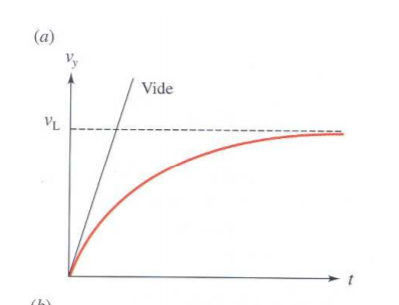
\includegraphics[scale = 0.8]{vitesse_limite}\\

Voici la formule permettant de la calculer :

\indent \indent $\frac{dv}{dt} = g-\frac{k\rho S}{m} v^2 \Rightarrow v(t) = v_L~\tanh(\frac{t}{T}),~T = \frac{v_L}{g}$

\indent \begin{itemize}
  \item S : section de la particule (surface)
  \item $\rho$ : masse volumique de l'air
  \item m : masse de la particule
  \item k : const proportionnelle au $C_X$, le coefficient de traînée (pas d'unité SI)
  \item $v_L$ : vitesse limite ($v_L = \sqrt{\frac{mg}{k\rho S}}$)
\end{itemize}
\newpage
\part{Inertie et mouvement à 2D}

\textbf{Définition de l'inertie}

L'inertie d'un corps est sa tendance à résister à toute variation de son état de mouvement.\\\\
\includegraphics[scale=0.65]{première_loi_de_Newton}\\\\\\
\textbf{Mouvement dans l'espace}\\

vecteur position $\overrightarrow{r}$\\\\
\indent \indent $\overrightarrow{r} = x\overrightarrow{i} + y\overrightarrow{j} + z\overrightarrow{k}$\\

vecteur déplacement $\Delta \overrightarrow{r}$:\\\\
\indent \indent $\Delta \overrightarrow{r} = \overrightarrow{r_2} - \overrightarrow{r_1} = \Delta x \overrightarrow{i} + \Delta y\overrightarrow{j}+\Delta z\overrightarrow{k}$\\

vitesse moyenne :\\\\
\indent \indent $\overrightarrow{v_{moy}} = \frac{\Delta\overrightarrow{r}}{\Delta t} = \frac{\Delta x}{\Delta t}\overrightarrow{i} + \frac{\Delta y}{\Delta t}\overrightarrow{j} + \frac{\Delta z}{\delta t}\overrightarrow{k}$\\

vitesse instantanée :\\\\
\indent \indent $\overrightarrow{v} = \displaystyle \lim_{\Delta t \to 0}\frac{\Delta \overrightarrow{r}}{\Delta t} = v_x\overrightarrow{i} + v_y\overrightarrow{j} + v_z\overrightarrow{k}$\\
\indent \indent où $v_x = \frac{\Delta x}{\Delta t},~v_y = \frac{\Delta y}{\Delta t},~v_z = \frac{\Delta z}{\Delta t}$\\

acceleration moyenne :\\\\
\indent \indent $\overrightarrow{a_{moy}} = \frac{\Delta \overrightarrow{v}}{\Delta t} = \frac{\overrightarrow{v_f} - \overrightarrow{v_i}}{t_f-t_i} = \frac{\Delta v_x}{\Delta t}\overrightarrow{i} + \frac{\Delta v_y}{\Delta t}\overrightarrow{j} +\frac{\Delta v_z}{\Delta t}\overrightarrow{k}$\\
\newpage

acceleration instantanée :\\\\
\indent \indent $\overrightarrow{a} = \displaystyle \lim_{\Delta t \to 0}\frac{\Delta \overrightarrow{v}}{\Delta t} = \frac{d\overrightarrow{v}}{dt} = a_x\overrightarrow{i} + a_y \overrightarrow{j} + a_z \overrightarrow{k}$\\
\indent \indent où $a_x = \frac{dv_x}{dt},~a_y = \frac{dv_y}{dt},~a_z = \frac{dv_z}{dt}$\\

équations du mouvement :\\\\
\indent \indent $\overrightarrow{v}(t) = \overrightarrow{v_0}\displaystyle \int^t_0 \overrightarrow{a}(t')dt'$\\
\indent \indent $\overrightarrow{r}(t) =  \overrightarrow{r_0} + \displaystyle \int^t_0 \overrightarrow{v}(t')dt'$\\\\

Ce qui est équivalent à\\\\
\indent \indent $\overrightarrow{v} = \overrightarrow{v_0} + \overrightarrow{a}t$\\
\indent \indent $\overrightarrow{r} = \overrightarrow{r_0} + \overrightarrow{v_0}t + \frac{\overrightarrow{a}t^2}{2}$\\\\\\
\textbf{Mouvement de projectile}

Composantes de l'acceleration : \\\\
\indent \indent $a_x = 0~~~~ a_y = -g = -9.81m/s^2$\\

equations de la cinematique pour un projectile :\\
\indent \indent $x = x_0 + v_{x_0}t$\indent \indent \indent$v_x = v_{x_0}$\\\\
\indent \indent $y = y_0 + v_{y_0}t-\frac{gt^2}{2}$\indent$v_y = v_{y_0}-gt$\\\\\\
\newpage
\noindent \textbf{Mouvement circulaire uniforme}\\
l'accélération instantanée est radiale et orientée vers le centre de la trajectoire : c'est l'accélération centripète.\\
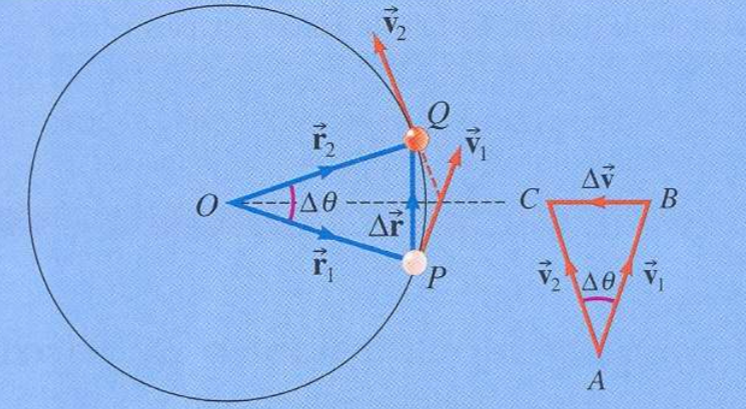
\includegraphics[scale=0.65]{MCU}\\

Seul la direction $\overrightarrow{v}$ change !\\\\
\indent \indent$\frac{||\Delta \overrightarrow{r}||}{r} = \frac{||\Delta \overrightarrow{v}||}{v}$\\\\
\indent \indent$||\Delta \overrightarrow{v}|| = \frac{v}{r}||\Delta \overrightarrow{r}||$\\\\

avec la limite de $\Delta t \to 0$, on a :\\
\indent \indent $a_r = \frac{v^2}{r}$\\

sous forme vectorielle :\\
\indent \indent $\overrightarrow{a_r} = -\frac{v^2}{r}\overrightarrow{u_r}$\\\\\\
\newpage
\noindent \textbf{Mouvement non-uniforme}\\\\

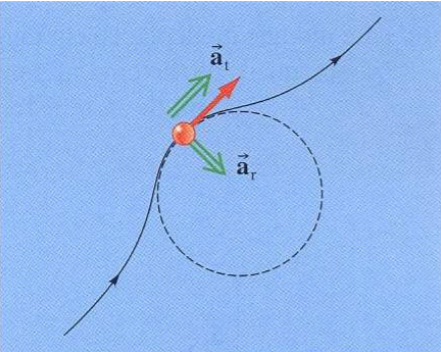
\includegraphics[scale=0.65]{MNU}\\

Les variations de vitesses de te modules correspondent à l'accélération tangentielle $a_t$ définie par\\\\
\indent \indent $a_t = \frac{dv}{dt}$\\

l'accélération résultante $a_r$ est la somme vectorielle de\\\\
\indent \indent $\overrightarrow{a} = \overrightarrow{a_r} + \overrightarrow{a_t}$\\

Et son module a est\\\\
\indent \indent $a = \sqrt{a_r^2 + a_t^2}$\\

\noindent \textbf{Mouvement circulaire non-uniforme}

Le mouvement sur une trajectoire circulaire est\\\\
\indent \indent $\overrightarrow{a} = \overrightarrow{a_r} + \overrightarrow{a_t} = -\frac{v^2}{r}\overrightarrow{u_r}+\frac{dv}{dt}\overrightarrow{u_{\theta}}$\\

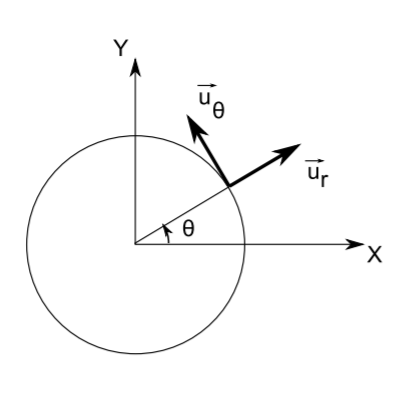
\includegraphics[scale = 0.65]{MCNU}\\

ici :
\begin{itemize}
\item $\overrightarrow{u_r}$ est le vecteur unitaire radial dirigé vers l'extérieur a partir du centre
\item $\overrightarrow{u_{\theta}}$ est le vecteur unitaire angulaire dirigé dans le sens de $\theta$
\end{itemize}
\textbf{Les référentiels inertiels}

Un référentiel est dit inertiel si un corps est soumis a une force résultante nulle ou elle reste au repos ou encore se déplace à vitesse constante.

remarques :
\begin{itemize}
\item tout système se d'éplaçant a vitesse constante par rapport à un référentiel inertiel est aussi un référentiel inertiel
  \item si l'acceleration d'une particule est nulle dans un référentiel inertiel alors elle est également nulle dans tout les autres référentiels inetiels plsu grands
\end{itemize}

\noindent \textbf{Vitesse relative}

Mouvement d’un corps : décrit par rapport à un référentiel. 
Besoin de déterminer le mouvement d’un corps par rapport à un autre corps

soit :\\
\indent \indent $\overrightarrow{r_{PA}}$ la position de la particule par rapport au référentiel A\\\\
\indent \indent $\overrightarrow{r_{PB}}$ la position de la particule par rapport au référentiel B\\\\
\indent \indent $\overrightarrow{r_{BA}}$ la position du référentiel B par rapport au référentiel A\\\\

on a :\\
\indent \indent $\overrightarrow{r_{PA}} = \overrightarrow{r_{PB}} + \overrightarrow{r_{BA}}$
\newpage
Si la particule P et le référentiel B se déplacent tous deux par rapport au référentiel A, on obtient :\\\\
\indent \indent $\overrightarrow{v_{PA}} = \overrightarrow{v_{PB}} + \overrightarrow{v_{BA}}$

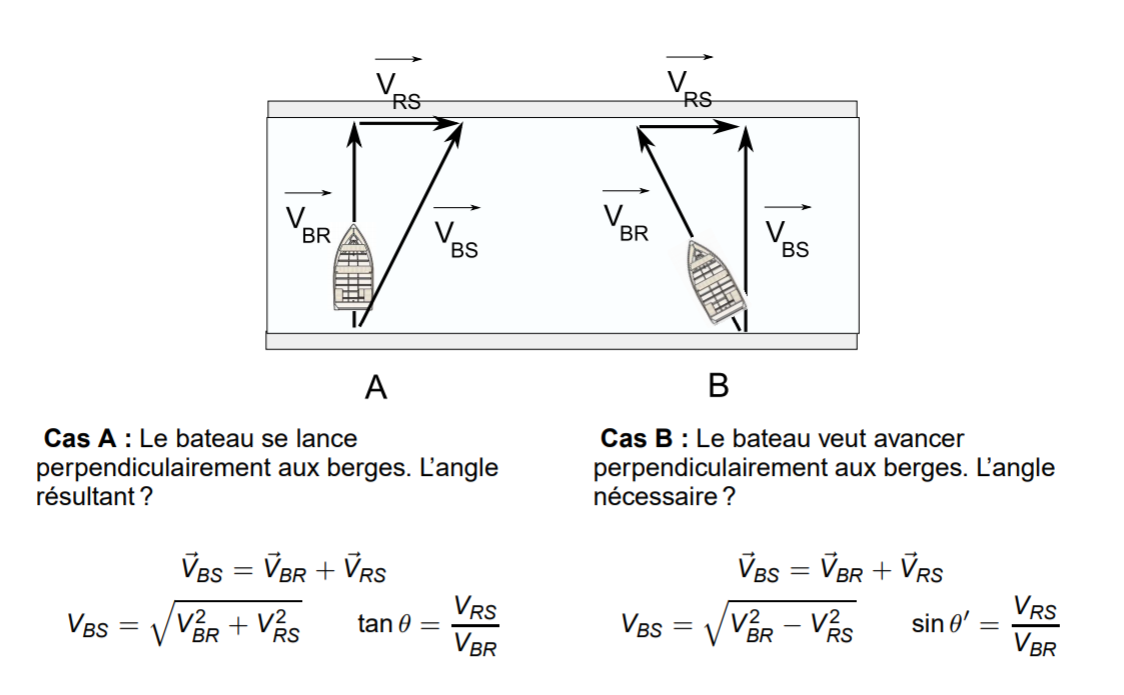
\includegraphics[scale=0.5]{vitesse_rel}\\
\newpage

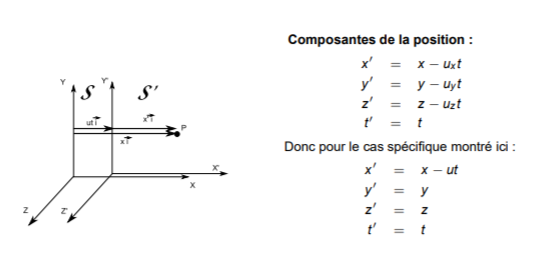
\includegraphics[scale=1]{transformation_gal}\\

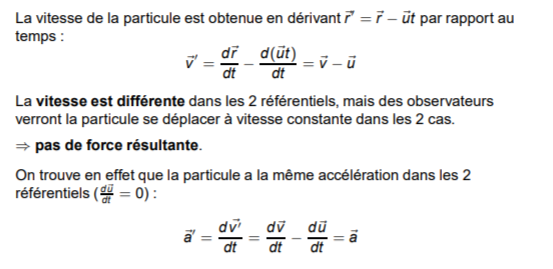
\includegraphics[scale=1]{transformation_gal_2}\\

\noindent \textbf{Principe de relativité Galilée-Newton :}

Les lois de la mécanique ont la même forme dans tous les référentiels d'inertie.
\newpage
\part{Dynamique de la particule 1}
\textbf{Première loi de Newton}

(voir partie 2)

\noindent \textbf{Force}

Caractéristiques :
\begin{itemize}
  \item Percues intuitivement comme une poussée ou une traction
  \item Invisible, on observe seulement ses effets
  \item Force de contact (corde, collision) ou action à distance (gravitation, électromagnetisme)
  \item La force est une vectorielle
\end{itemize}

\noindent \textbf{Masse}

La masse d'un corps est la mesure de son inertie, càd de sa résistance à la variation de vitesse (grandeur scalaire)

\textbf{unité SI :}\\
\indent \indent L'unité du SI est le newton noté $N$\\
\indent \indent elle s'exprime $1N = 1kg m/s^2$\\µ

\noindent \textbf{Seconde loi de Newton}\\

La force résultante $\Sigma \overrightarrow{F}$ agissant sur une particule de masse m produit par une accélération $\overrightarrow{a}=\frac{\Sigma \overrightarrow{F}}{m}$ de même orientation que la force résultante\\\\

on en déduit alors la formule suivante :\\\\
\indent \indent $\Sigma \overrightarrow{F} = m\overrightarrow{a}$
\end{document}
